\bigsection{A New Framework}
\label{sec:framework}%

The two prominent frameworks for a parameterized analysis of complexity are those of \citeauthor{downey1999parameterized} and of \citeauthor{flum2006parameterized}, introduced in Section~\ref{sec:parameterized_complexity_theory}.
Both are rooted in computational complexity theory and they each have their own theoretical shortcomings.
We shall build a more universal framework and resolve the shortcomings of these earlier frameworks that we have identified in Section~\ref{sec:parameterized_complexity_theory}.

Several forms of complexity that could be related to parameters of instances were listed in Section~\ref{sec:history}.
In the next chapter, we shall use our new framework in a more concise analysis of these forms of complexity.
This shows that our framework can be applied outside the theory of computational complexity.
Indeed, our framework serves as a mathematical model of complexity that is applicable to a broad range of complexities.
Still, all of our notions of complexity are involved with computation in one way or another.
Our framework is therefore not limited to a notion of a \emph{parameterization}.
It also includes a notion of a \emph{parameterized procedure}, which is a computation that takes as input not just an instance, but also a parameter value.

\subsubsection{Desiderata}
The picture that emerges from Section~\ref{sec:history} is that a parameter of a problem instance is any of a collection of related properties the object may have.
For instance, a graph may have any number of vertices, hence the number of vertices in a graph is a parameter of the graph.
Another parameter of a graph would be its number of edges.
This corresponds to the property schema that we have seen in Example~\ref{ex:edges}.
Each specific property we shall refer to as a \emph{parameter value}.
Hence, if the number of edges is the parameter at hand, then `$9$' is a possible parameter value, expressing that a graph has $9$~edges.
A \emph{parameterization}, then, should link an instance~$x$ to the parameter values that apply to~$x$.
Note that we shall use the term \emph{parameter} loosely so that it encompasses the various meanings it has in the literature.
The terms \emph{parameter value} and \emph{parameterization} will be made precise shortly and we shall never use them informally.
By making parameterizations \emph{independent} of decision problems, we resolve one of the two shortcomings we identified in the framework of \citeauthor{downey1999parameterized}.
Namely, a parameterized analysis of the complexity of classical decision problems will be possible.

In our framework, we want to relate notions of complexity to parameter values.
In order for every instance to have a complexity assigned to it, we want parameterizations to link each instance to at least one parameter value.
We summarize this desire by saying that we want parameterizations to be, in some sense, \emph{total}.
Wanting to have a complexity assigned to all instances can be motivated by an engineering view on taking measurements.
We feel that if instances are bigger than your measuring device, you need a bigger measuring device.
In our case, we want to use parameterizations as a measuring device for measuring complexity.
Requiring parameterizations to be total makes sure that we shall be able to deal with nonmembers of decision problems.
This resolves the other shortcoming we identified in the framework of \citeauthor{downey1999parameterized}.

Additionally, we desire parameterizations, and in particular parameter values, to be \emph{general}.
We have seen that if we restrict each parameter value to be a natural number, as with \citeauthor{flum2006parameterized}, the interplay between parameter values cannot be expressed.
In our framework, we want to support even parameters where the parameter values are not ordered linearly.
However, as we shall see, we do well to put in place at least some requirements regarding an order on parameter values.

Parameter values naturally have a stronger-than order given by set inclusion:
If the set of instances that have a property~$P$ is included in the set of instances that have property~$Q$, then property~$P$ is stronger than property~$Q$.
In our graph example, we need to generalize the properties we look at somewhat to make this order visible.
The set of graphs that have $4$~vertices is disjoint from the set of graphs that have $5$~vertices.
However, the set of graphs that have \emph{at most} $4$~vertices is a subset of the set of graphs that have \emph{at most} $5$~vertices.
In that sense, the former property is stronger than the latter.
This order works for more diverse collections of parameter values as well.
For example, every graph that has at most $4$~vertices has at most $9$~edges.
Thus, again, the former is a stronger property than the latter.
Conversely, the property of having at most $9$~edges is weaker than the property of having at most $4$~vertices.
At the same time, the property of having at most $9$~edges is incomparable to the property of having at most $5$~vertices.
The full graph with $5$~vertices has $10$~edges, and an empty graph with $6$~vertices has no edges.

Let us take a look at what this order can mean for computations that involve parameters.
Suppose we have some function that we can compute on graphs with a given property, say graphs that have at most $4$~vertices.
Often, this function can be \emph{extended} to cover graphs with a weaker property, say graphs that have at most $5$~vertices.
If we keep on extending our function to be applicable to graphs with more and more vertices, we approach a function that works on all graphs.
We desire our parameterizations to be \emph{consistent} in that the function we end up with does not depend on the way we go from property to property.

\begin{example}
\label{ex:inconsistent}%
  Consider the following two parameters concerning a graph~$G$, where $e$ and~$w$ represent parameter values corresponding to each of the parameters.
  \begin{enumerate}
  \item The number of edges in~$G$ is at most~$e$.
  \item The number of \bits{1}s in the representation of the number of vertices in~$G$ as a binary string is at most~$w$.
  \end{enumerate}
  Admittedly, the second parameter is rather contrived, but its behavior with respect to the first parameter is of interest.
  For no values of $e$ and~$w$ is either parameter weaker than the other.
  However, for both parameters we find that if we keep increasing the parameter value, we will eventually include any graph.

  Now, suppose we want to build a function by defining it on graphs with a certain property and then iteratively extending it to weaker properties.
  Once we have chosen one of our two parameters, we must stick to that choice.
  This is so because, as we saw, for no values of $e$ and~$w$ is either parameter weaker than the other.
  As a result, nothing stops us from building completely different functions depending on what parameter we choose to start with.
\end{example}

We want to prevent situations such as in the example above.
Concretely, we want to disallow parameterizations that incorporate just the two parameters mentioned in the example, and nothing else.
One way to achieve consistency, is by requiring that for every two parameter values, there is another that is weaker than both.

\subsubsection{Definitions}
In our framework, we want to allow parameter values to have all sorts of structure.
To make this possible, we choose to make as few assumptions about parameter values as necessary.
One thing we shall assume is that in any parameterized context, the set of possible parameter values is countable.
This assumption has the effect that parameter values can be encoded as binary strings and can be processed algorithmically.
In fact, we shall leave any interpretation of parameter values to the user of a parameterization and proceed as if parameter values \emph{are} binary strings.
Thus, we take care of the desire to make parameterizations, and parameter values in particular, as \emph{general} as possible.

This leaves us with three desiderata to consider when defining parameterizations.
Namely, a parameterization should be \emph{independent}, \emph{total} and \emph{consistent}.
The first of these can be met simply by avoiding any dependence on a decision problem in the definition of a parameterization.
For the other two, we look at the sets of instances that each parameter value identifies.
If a parameter value, a string~$k$, represents the property of having at most $4$~vertices, then $k$ identifies the set of graphs with at most $4$~vertices.
This suggests defining a parameterization as a family of sets indexed by parameter values.
\begin{definition}
  A \defkey{parameterization} is a directed cover of~$\binary^+\!$, indexed by $\binary^+\!$.
  The elements of a parameterization are called its \defkeyat{slice}{slices}.
\end{definition}

By requiring a parameterization to be a cover of~$\binary^+\!$, any instance is present in at least one slice of a parameterization.
Thus, this definition of parameterizations satisfies our desire of parameterizations being \emph{total},
The requirement that a parameterization is directed makes sure that situations as in Example~\ref{ex:inconsistent} cannot occur and we have a form of \emph{consistency}.

For strings, the most-used parameter in computer science must be the \emph{length}.
This parameter can be represented by a parameterization.
\begin{example}
\label{ex:length_parameterization}%
  The \defkey{length parameterization} \parencite[see also][Example~1.6]{flum2006parameterized} is defined as
  \begin{equation*}
    (\{x \st \length{x} \le \asNat(k)\})_{k \in \binary^+}.
  \end{equation*}
  In this parameterization, depicted in Figure~\ref{fig:length_parameterization}, the parameter value~$k$ acts as an upper bound on the lengths of instances.
  We remark that when instances are not just strings, but more structured objects such as graphs, a \enquote{length} is only defined in light of an encoding.
  \begin{figure}
    \centering
    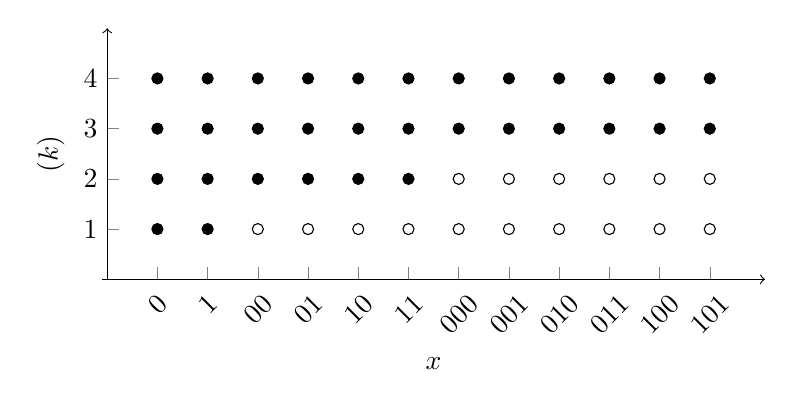
\begin{tikzpicture}
      \begin{axis}[
        width=10cm,
        axis equal image=true,
        axis lines*=middle,
        axis line style={->},
        xlabel={$x$},
        ylabel={$\asNat(k)$},
        xtick={1,2,...,12},
        xticklabels={\bits{0},\bits{1},\bits{00},\bits{01},\bits{10},\bits{11},\bits{000},\bits{001},\bits{010},\bits{011},\bits{100},\bits{101}},
        xticklabel style={rotate=45},
        ymin=0,
        ymax=5,
        ytick={1,2,...,4},
      ]
        \foreach \k in {1,2,...,4} {
          \addplot[
            only marks,
            mark=*,
            samples at={1,2,...,\k < 3 ? 2^(\k+1)-2 : 12}
          ] {\k};
          \addplot[
            only marks,
            mark=o,
            samples at={2^(\k+1)-1,2^(\k+1),...,12}
          ] {\k};
        }
      \end{axis}
    \end{tikzpicture}
    \caption{
      An initial segment of the length parameterization.
      Filled marks indicate members of the slices of the parameterization, whereas open marks indicate nonmembers.
      Note that the elements of the parameterization, depicted as rows in the figure, are finite sets.
      Furthermore, the inclusion order on the elements of the parameterization matches the natural enumeration order on the set~$\binary^+$ of parameter values.
      Neither of these two properties is required to hold for parameterizations in general.
    }
    \label{fig:length_parameterization}
  \end{figure}
\end{example}

Parameterizations are intended to also measure structures of instances other than their lengths.
Note that the length of a string is commonly associated with the symbol~$n$.
To highlight the role of parameterizations as more general measures of structure, we use a similar-looking symbol for parameterizations:~$\eta$.
By convention from parameterized complexity theory, we shall mostly use~$x$ for instances and~$k$ for parameter values.
The slice of a parameterization~$\eta$ that corresponds to a parameter value~$k$ is denoted by~$\eta_k$.

In our framework, parameter values are mapped to sets of instances.
In this regard, our framework differs from that of~\textcite{flum2006parameterized}, where instances are mapped to parameter values.
Of course, given a parameterization~$\eta$ and an instance~$x$, we can consider the set $\{k \st x \in \eta_k\}$.
These are the parameter values that the parameterization~$\eta$ links to the instance~$x$.
Contrary to \citeauthor{flum2006parameterized}, we make no demands regarding the computability of such a mapping from instances to parameter values.

Recall that parameter values in the frameworks of \textcite{downey1999parameterized} and of \textcite{flum2006parameterized} are typically natural numbers.
This allows us to compare parameter values assigned to an instance by different parameterizations using the usual less-than-or-equal-to order~\parencite{komusiewicz2012new}.
In our more general framework, where instances are associated with sets of binary strings, comparing parameterizations is less straightforward.
To facilitate a comparison between parameterizations, we shall look at the length, in bits, of the shortest parameter value for some given instance.
\begin{definition}
  Given a parameterization~$\eta$, the \defkeyat{m@$\mu_\eta$}{minimization function} of~$\eta$ is defined as
  \begin{equation*}
    \mu_\eta(x) \deq \min\{\length{k} \st x \in \eta_k\}.
  \end{equation*}
\end{definition}
Note that $\mu_\eta$ minimizes with respect to the length of parameter values and not with respect to the inclusion order on the slices of the parameterization.

Like in the framework of \textcite{downey1999parameterized}, in our framework an instance can be associated with multiple parameter values.
Therefore, a parameterized analysis of decision problems requires a generalization of decision procedures.
A parameterized decision procedure, or \defkeyat{parameterized procedure|(}{parameterized procedure} for short, is a special kind of procedure that takes two arguments.
In line with ordinary decision procedures, we require parameterized procedures to be total, meaning that their computation terminates on all possible inputs.
However, we do not require the output of a parameterized procedure to be either \bits{1} or~\bits{0}, representing the judgments `yes' and `no'.
Any other output a parameterized procedure produces we interpret as~\bits{?}, representing the judgment `unknown'.
In summary, a parameterized procedure is a procedure that takes two strings as input and produces an output in the set $\{\bits{1}, \bits{0}, \bits{?}\}$.\indexkey{parameterized procedure|)}

We would like to associate parameterized procedures to sets in a way similar to how decision procedures are associated to sets.
In the presence of parameterizations, this is possible for some parameterized procedures.
\begin{definition}
  A parameterized procedure~$\phi$ \defkeyat{parameterized procedure!convergence}{converges} to a set~$A$ on a parameterization~$\eta$ if, for all strings $x$ and~$k$, we have
  \begin{equation*}
    x \in \eta_k \:\implies\: \phi(x, k) = A(x).
  \end{equation*}
\end{definition}

A parameterization~$\eta$ is consistent in the sense that it is directed.
Therefore, when a parameterized procedure~$\phi$ converges to a set~$A$ on~$\eta$, we can think of~$A$ as a \emph{limit} of~$\phi$.
However, the set to which a parameterized procedure converges may depend on the parameterization.
\begin{example}
\label{ex:convergence}%
  Consider the parameterizations $\eta$ and~$\zeta$ given by
  \begin{equation*}
    \eta_k \deq \begin{cases}
      \binary^+	& \text{if $k = \bits{0}$}, \\
      \emptyset	& \text{otherwise},
    \end{cases}
    \qquad\text{and}\qquad
    \zeta_k \deq \begin{cases}
      \emptyset	& \text{if $k = \bits{0}$}, \\
      \binary^+	& \text{otherwise},
    \end{cases}
  \end{equation*}
  and the parameterized procedure~$\phi$ given by
  \begin{equation*}
    \phi(x, k) \deq \begin{cases}
      \bits{1}	& \text{if $k = \bits{0}$}, \\
      \bits{0}	& \text{otherwise}.
    \end{cases}
  \end{equation*}
  These definitions are so that $\phi$ converges to~$\binary^+$ on~$\eta$, but to~$\emptyset$ on~$\zeta$.
\end{example}

The above example shows that a parameterized procedure can have multiple limits.
One way to enforce the limit of a parameterized procedure to be unique is by strengthening our notion of convergence.
We do so by turning to a special kind of parameterizations.
\begin{definition}
  A parameterization~$\eta$ is \defkeyat{parameterization!point-cofinite}{point-cofinite} if each instance $x \in \binary^+$ is excluded from only finitely many slices of~$\eta$.
\end{definition}

The length parameterization of Example~\ref{ex:length_parameterization} is an example of a point-cofinite parameterization.
With point-cofinite parameterizations, a situation as in Example~\ref{ex:convergence} cannot occur.
A parameterized procedure~$\phi$ may converge on two different point-cofinite parameterizations, but the set to which $\phi$ converges will be the same either way.
In other words, as far as convergence on point-cofinite parameterizations is concerned, the limit of a parameterized procedure, if it exists, is unique.
Therefore, when dealing with convergence in the context of point-cofinite parameterizations, we need not mention a point-cofinite parameterization explicitly.
We may simply say that a parameterized procedure~$\phi$ converges to a set~$A$.
This then means that there exists a point-cofinite parameterization~$\eta$ such that $\phi$ converges to~$A$ on~$\eta$.
The existence of a set~$A$ to which a parameterized procedure converges is is hence a property of the parameterized procedure alone.
\begin{definition}
\label{def:convergent}%
  A parameterized procedure~$\phi$ is \defkeyat{parameterized procedure!convergence}{convergent} if there is a set to which it converges.
  In more detail, this means $\phi$ is convergent if there is a set~$A$ and a point-cofinite parameterization~$\eta$ such that $\phi$ converges to~$A$ on~$\eta$.
\end{definition}

Suppose a parameterized procedure~$\phi$ converges to a set~$A$ on a point-cofinite parameterization~$\eta$.
Because $\eta$ is point-cofinite, the set~$A$ does not depend on the specifics of~$\eta$, but only on the fact that it is point-cofinite.
This does not mean that whenever for some instance~$x$ and parameter value~$k$ we have $\phi(x, k) = \bits{1}$, we can conclude that $x$ is a member of~$A$.
Likewise, whenever we have $\phi(x, k) = \bits{0}$, we cannot conclude that $x$ is not a member of~$A$.
All we know is that for each instance~$x$ there are only finitely many parameter values~$k$ such that $\phi(x, k)$ is not in agreement with membership of~$x$ in~$A$.
In other words, we do not \emph{know} when the output of~$\phi$ is correct, only that it will eventually be correct.

An alternative way to enforce that a parameterized procedure has only one limit set, is by requiring the procedure to know when it is correct.
A parameterized procedure~$\phi$ knows when it is correct if there is a set~$A$ such that, for all $x$ and~$k$, the output of $\phi(x, k)$ is either \bits{?} or~$A(x)$.
In order for this set~$A$ to be unique, we require that the procedure~$\phi$ must converge to~$A$ on some parameterization~$\eta$.
Because the output of~$\phi$ is never wrong, we can derive a family of sets from it that could potentially serve as such a parameterization~$\eta$.
\begin{definition}
\label{def:direct}%
  A parameterized procedure~$\phi$ is \defkeyat{parameterized procedure!direct}{direct} if
  \begin{equation*}
    (\{x \st \phi(x, k) \neq \bits{?}\})_{k \in \binary^+}
  \end{equation*}
  is a parameterization on which $\phi$ converges to some set~$A$.
\end{definition}

A parameterized procedure can be convergent, direct, neither, or both.
In the parameterized version of computational complexity theory, parameterized procedures that are both convergent and direct often emerge quite naturally.
\begin{example}
\label{ex:clique_vc}%
  \indexkey{Clique@\pr{Clique}}%
  In Section~\ref{sec:parameterized_complexity_theory}, we have looked at a parameterized analysis of the \pr{Clique} problem,
  \begin{align*}
    \pr{Clique} \deq \{(G, l) \st &\text{there is a set of at least $l$ vertices of the graph $G$ in which} \\
          &\text{each pair of vertices is connected by an edge}\},
  \end{align*}
  with respect to the minimum vertex cover size.
  We found that in the framework of \citeauthor{downey1999parameterized}, such an analysis was not very natural:
  It required the construction of an intricate parameterized decision problem where the instances of the form $(G, l)$ were replaced by structures of the form $\pair{(G, l)}{k}$.

  In our framework, we can consider the unmodified \pr{Clique} problem with respect to the point-cofinite vertex cover parameterization
  \begin{equation*}
    \eta \deq (\{(G, l) \st \text{$G$ has a vertex cover of at most $\asNat(k)$ vertices}\})_{k \in \binary^+}.
  \end{equation*}
  In the framework of \citeauthor{downey1999parameterized}, the \pr{Clique} problem parameterized by the minimum vertex cover size was found to be fixed-parameter tractable.
  For our framework, this means that there is a direct parameterized procedure~$\phi$ such that
  \begin{itemize}
  \item $\phi$ converges to \pr{Clique} on~$\eta$, and
  \item for some function~$f$ and constant~$c$, the running time of~$\phi$ on any instance of length~$n$ and parameter value~$k$ is at most $f(k) \cdot n^c$.
  \end{itemize}
  Note that because $\eta$ is point-cofinite, this procedure~$\phi$ is not only direct, but also convergent.

  Thus, an analysis of fixed-parameter tractability can be performed in our framework.
  Moreover, this is possible without resorting to intricate parameterized decision problems and the parameterization can be reused for other problems.
  We remark that a more fundamental definition of fixed-parameter tractability will be given in Section~\ref{sec:tractability:stratified}.
\end{example}

When the parameter value is held fixed, the behavior of a direct parameterized procedure can be thought of as an approximation of a decision procedure.
Indeed, such procedures are of interest also without any parameter values playing a part.
\begin{definition}
\label{def:approximation}%
  Given a function $t$, a procedure~$\phi$ is a \defkeyat{approximation@$t$-approximation}{$t$"~approximation} for a set~$A$ if it satisfies, for every string~$x$,
  \begin{itemize}
  \item $\phi(x)$ outputs either \bits{?} or $A(x)$, and
  \item $\phi$ terminates on input $x$ within $t(\length{x})$ steps.
  \end{itemize}
  A $t$"~approximation~$\phi$ is said to \emph{decide} the elements of its \defkeyat{approximation@$t$-approximation!domain}{domain}
  \begin{equation*}
    \dom(\phi) \deq \{x \st \phi(x) \neq \bits{?}\}.
  \end{equation*}
\end{definition}

The \defkeyat{approximation@$t$-approximation!polytime}{polytime-approximations} \parencite{ko1981completeness,balcazar1985bi-immune} are $t$"~approximations where $t$ is a polynomial.
Likewise, a procedure is an \defkeyat{approximation@$t$-approximation!O(f)@$\bigO(f)$}{$\bigO(f)$"~approximation} if it is a $t$"~approximation for some $t \in \bigO(f)$.
The fact that the bound is a bound on the running time is left implicit.
For time-constructible functions~$t$, the domain of a $t$"~approximation is decidable in time~$t$.
In particular, the domain of a polytime-approximation is in \cl{P}, without an increase in the degree of the polynomial.
The domain of a polytime-approximation is also known as the \emph{definite part} of the approximation~\parencite{ko1981completeness}.
